\documentclass[12pt]{article}
\usepackage{graphicx}
\usepackage{amssymb}
\usepackage{epstopdf}
\usepackage{amsmath}
\usepackage{multicol}
\usepackage{tcolorbox}
\usepackage{geometry}
\usepackage{enumitem}
\usepackage{fancyhdr}

\DeclareGraphicsRule{.tif}{png}{.png}{`convert #1 `dirname #1`/`basename #1 .tif`.png}

\textwidth = 6.5 in
\textheight = 9 in
\oddsidemargin = 0.0 in
\evensidemargin = 0.0 in
\topmargin = -23pt
\headheight = 0.0 in
\headsep = 0.0 in
\parskip = 0.2in
\parindent = 0.0in
\pagestyle{fancy}
\pagenumbering{gobble}

\newtheorem{theorem}{Theorem}
\newtheorem{corollary}[theorem]{Corollary}
\newtheorem{definition}{Definition}
%\includegraphics [height=50mm, width=50mm]{PathInt.jpg}
\title{Title} 

\begin{document}
%INSTRUCTOR NOTES

 Name:
 \begin{center}\large{3.3 Product and Quotient Rules}\end{center}


\begin{tcolorbox}

\textbf{Product Rule:} $\displaystyle \frac{d}{dt} \left[f(t)g(t)\right]=$\\
\vspace{10mm}

\textbf{Quotient Rule:} $\displaystyle \frac{d}{dt} \left[\frac{f(t)}{g(t)}\right]=$\\
 \vspace{5mm}

\end{tcolorbox}

\begin{enumerate}
\item Compute the following derivatives.

	\begin{multicols}{2}
	\begin{enumerate}[itemsep=1.6cm]
	\item $\displaystyle \frac{d}{dx}\left(\sqrt{x}2^{x}\right)=$

	\item $\displaystyle \frac{d}{dx}\left(\left(x^{2}+3\right)e^{x}\right)=$

	\item $\displaystyle \frac{d}{dx}\left(\frac{x}{e^{x}}\right)=$

	\item $\displaystyle \frac{d}{dx}\left(\frac{x+1}{x^{2}} \right)=$
	
	\item $\displaystyle \frac{d}{dx}\left(\frac{3^xx^4}{3x-2} \right)=$
	
	\item $\displaystyle \frac{d}{dx}\left( 2^x 3^x 4^x \right)=$

	\end{enumerate}
	\end{multicols}
\vfill
\item Suppose $f(x)$ is the curved, dotted line function and $g(x)$ is the piecewise-straight solid function. If $\displaystyle h\left(x\right)=f\left(x\right)g\left(x\right)$, find the following, or explain why it doesn't exist.

\noindent\begin{minipage}{0.3\textwidth}% adapt widths of minipages to your needs
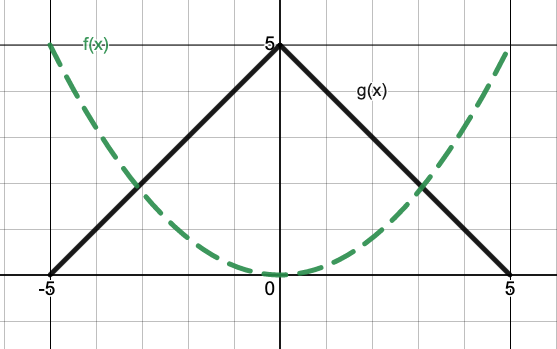
\includegraphics[scale=.4]{3_3_piecewise}
\end{minipage}%
\hspace{40mm}
\begin{minipage}{0.6\textwidth}
	(a) $\displaystyle h'\left(-2\right)$\\
	
	\vspace{10mm}
	 (b) $\displaystyle h'\left(0\right)$\\
	 
	\vspace{10mm}
	(c) $\displaystyle h'\left(2\right)$\\
\end{minipage}
\newpage
~
\item The density of veins on leaves tells us about a region's past climate. Scientists measure vein density, $V$, in mm per mm$^2$, by estimating the average distance, $x$, in mm, between veins on a leaf, and using the formula:

$$V=f(x)=\frac{0.629}{x}+1.073$$
	\begin{enumerate}
	\item Calculate $f'(x)$ using the power rule.
	\vfill
	\item Calculate $f'(x)$ using the quotient rule.
	\vfill
	\item What are the units of $f'(x)$?
	\vfill
	\item Calculate $f'(x)$ and interpret the meaning of your answer in practical terms.
	\end{enumerate}
\vfill
\item For what intervals is $\displaystyle g\left(t\right)=\frac{1}{t^{2}+1}$ concave down? Check using Desmos.
\vfill
\item Find a possible formula for a function $y=f(x)$ such that $f'(x)=10x^{9}e^{x}+x^{10}e^{x}$. Are other formulas possible?
\vfill

\end{enumerate}
\end{document} 

%%%%%%%%%
\begin{tcolorbox}
\textbf{Warm-up: } Solve the following equations for $t$.
\begin{multicols}{2}
\begin{enumerate}
\item $(t+1)^2=9$
\item $tx+x^2=5$
\end{enumerate}
\end{multicols}
\end{tcolorbox}

MINIPAGE
\noindent\begin{minipage}{0.3\textwidth}% adapt widths of minipages to your needs
try 1
\end{minipage}%
\hspace{40mm}
\begin{minipage}{0.6\textwidth}
a) $f'(2)=$\\\

b) $f'(4)=$\\

c) $f'(6)=$\\

d) $f'(7)=$\\

e) $f'(8)=$
\end{minipage}
